\input{prefix}  % Place all packages in the prefix file

% Set up document info
\title{\Huge\textbf{Tissue Engineering \\ - Motta -}}
\author{
  Stefano Cretti\\
  \small telegram: \href{https://t.me/StefanoCretti}{@StefanoCretti} \\[3pt]
\small Github: \href{https://github.com/StefanoCretti/TissueEngineering.git}{https://github.com/StefanoCretti/TissueEngineering.git}}

\begin{document}
\maketitle
\tableofcontents

    \input{chapters/01_generalInfo}
    \input{chapters/02_basicsOfTissueEngineering}
    \graphicspath{{chapters/06_images/}}
\chapter{Biocompatibility}

\section{Introduction}
Biocompatibility is an essential aspect to take into consideration for the specification of the medical device that is being designed.
Before building a scaffold or a biological device its time, location and individual in which it will be used need to be defined.
A scaffold to be useful should activate specific cellular function and reflect and exploit the different mechanical and chemical properties of the tissue in which it will be implanted.
Because of this a scaffold it's designed taking into account the specific region in which it will be implanted considering the cell population and kind of injury among other parameters.
Cells are the building blocks of biology and they can read the information coming from the external environment.
Specific gene expression is activated in cells given external signalling molecules.
This makes it evident that the environment reaches the cell through chemical and mechanical stimuli.
Because of this scaffold are not self-sufficient entities: they are bioactive and need to collaborate with environment, cells and the extracellular matrix to perform their function.

	\subsection{Parameters defining biological outcome}
	The biological outcome that will be obtained then depends on a list of parameters which, once defined allow for the creation of a scaffold capable of regenerating the injured tissue.
	This parameters are:

	\begin{multicols}{2}
		\begin{description}
		\item[Porosity] is extremely important for cell migration.
			The material should be 3D for the cells, meaning that the scaffold should allow and promote cell adhesion, growth and migration.
		\item[Mechanical properties] are different for each tissue, the scaffold should both resist physical stress and provide the correct stimulus that the cells need to grow, adhere, migrate and differentiate.
		\item[Surface] modification is often referred to the functionalization of the scaffold through the addition of proteins or sequence of aminoacids to increase adherence.
		\item[Antibiotic/antiviral] drugs release system, to control chronic inflammation and possible infections.
		\item[Surface topography] may be smooth or rough for example.
		\end{description}
	\end{multicols}

\section{Guided tissue regeneration}
\begin{figure}[ht]
\centering
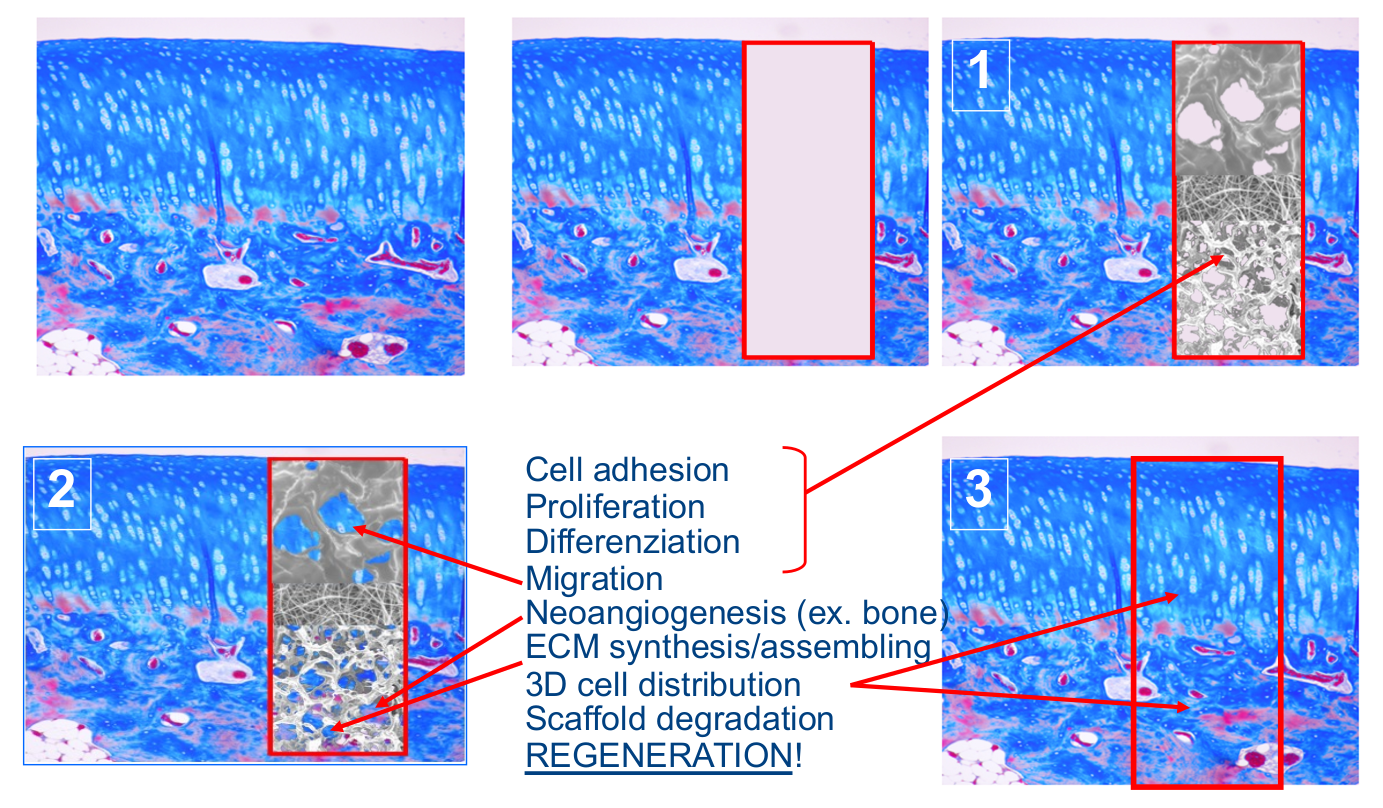
\includegraphics[width=0.5\textwidth]{cartilage.png}
\caption{\label{fig:cartilage}}
\end{figure}
In the figure we can see articular cartilage, an intermidiate zone and bone. These three different tissues present differences in vasculartion, cell organization (in cartilage cells live in lacuna, where migration and proliferation are downregulated) and innervation.
\\
If the damage reaches the bone (which happens most of the times, because the cartilge does not have innervation, while bone does), the scaffold needs to account for different types of tissue. A multicomponent scaffold is designed, something that upregulates angiogenesis in the bone and downregulates it in the cartilage, that has high resistance to mechanical stimulations (cartilage has more water, material reaching water with hydrofilic properties). It should also provide for an enviroment for osteoblasts, lacunae for cartilage cells, space for nerves, vascularity and migration. It also needs to have different degradation times.
\\
The next step is check the biocompatibility, which will have an impact on cell adhesion, proliferation, differentiation, and also migration; on neoangiogenesis (spefic function) etc. Difference between regeration and repair (no/presence of scar tissue).

\section{The principles of tissue engineering}
\begin{figure}[ht]
\centering
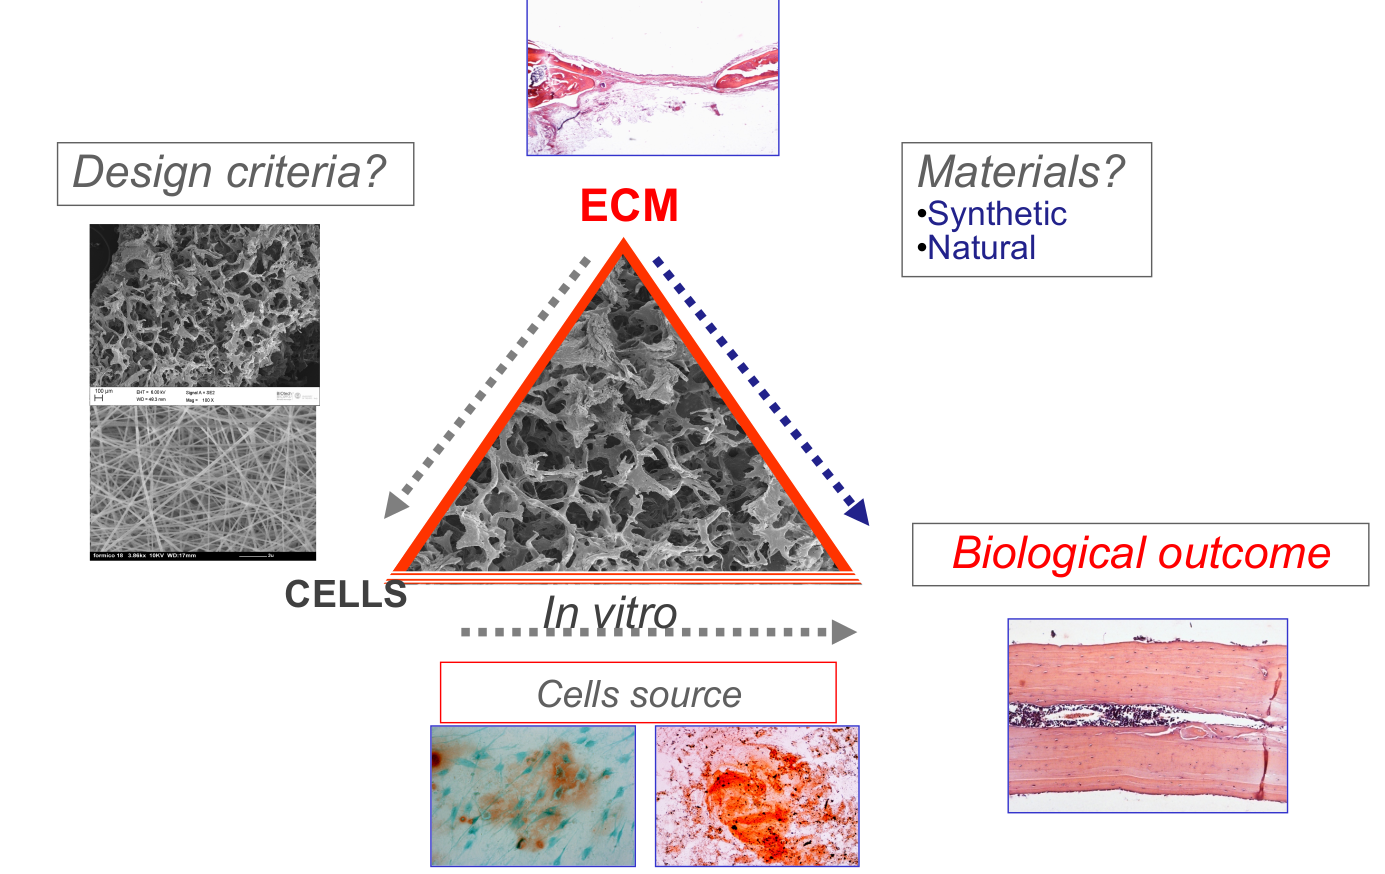
\includegraphics[width=0.5\textwidth]{triangolo.png}
\caption{\label{fig:triangle}}
\end{figure}

A tissue engineering process is composed by three steps:

\begin{multicols}{3}
	\begin{itemize}
		\item Design.
		\item Material choice.
		\item In vitro and in vivo testing.
	\end{itemize}
\end{multicols}

Tissue engineering implements a multidisciplinary strategy and the advance in materials' science and biology drastically improve the success of scaffold application.
Just consider how much the progressive knowledge in biology incremented the one in biocompatibility.
For example, M1 and M2 macrophages were only discovered in 2000.
But also the invention of polymers that can change their activity based on the environment (thermo/ph responsive), instructional (functionalization, e.g. with peptides that can control the cells' fate) and that can have specific mechanical strength and function (mechanical signalling).
In particular, the materials that can satisfy those requirements are considered 4th generation "biological regenerative biomaterials".
\\
Biomaterial need to be stable and inert in the beginning to be able to deliver drugs, to be used to print organ and used for cell therapies.
The hope for the future is to develop also diagnostic systems and to implant electronic devices, but one thing must always be present: biocompatibility.

	\subsection{Biocompatibility: a definition}
	At first, a material is biocompatible when inert, a ghost in the body: "the total absence of interaction between the material and the tissues".
	The minimal reaction to the foreign body was preferred, meaning no (or low) inflammatory reaction, no immuno-response.
	Definition focused on the body reaction to the implant and what was required was simply the chemical stability by the time.
	\\
	\begin{figure}[ht]
\centering
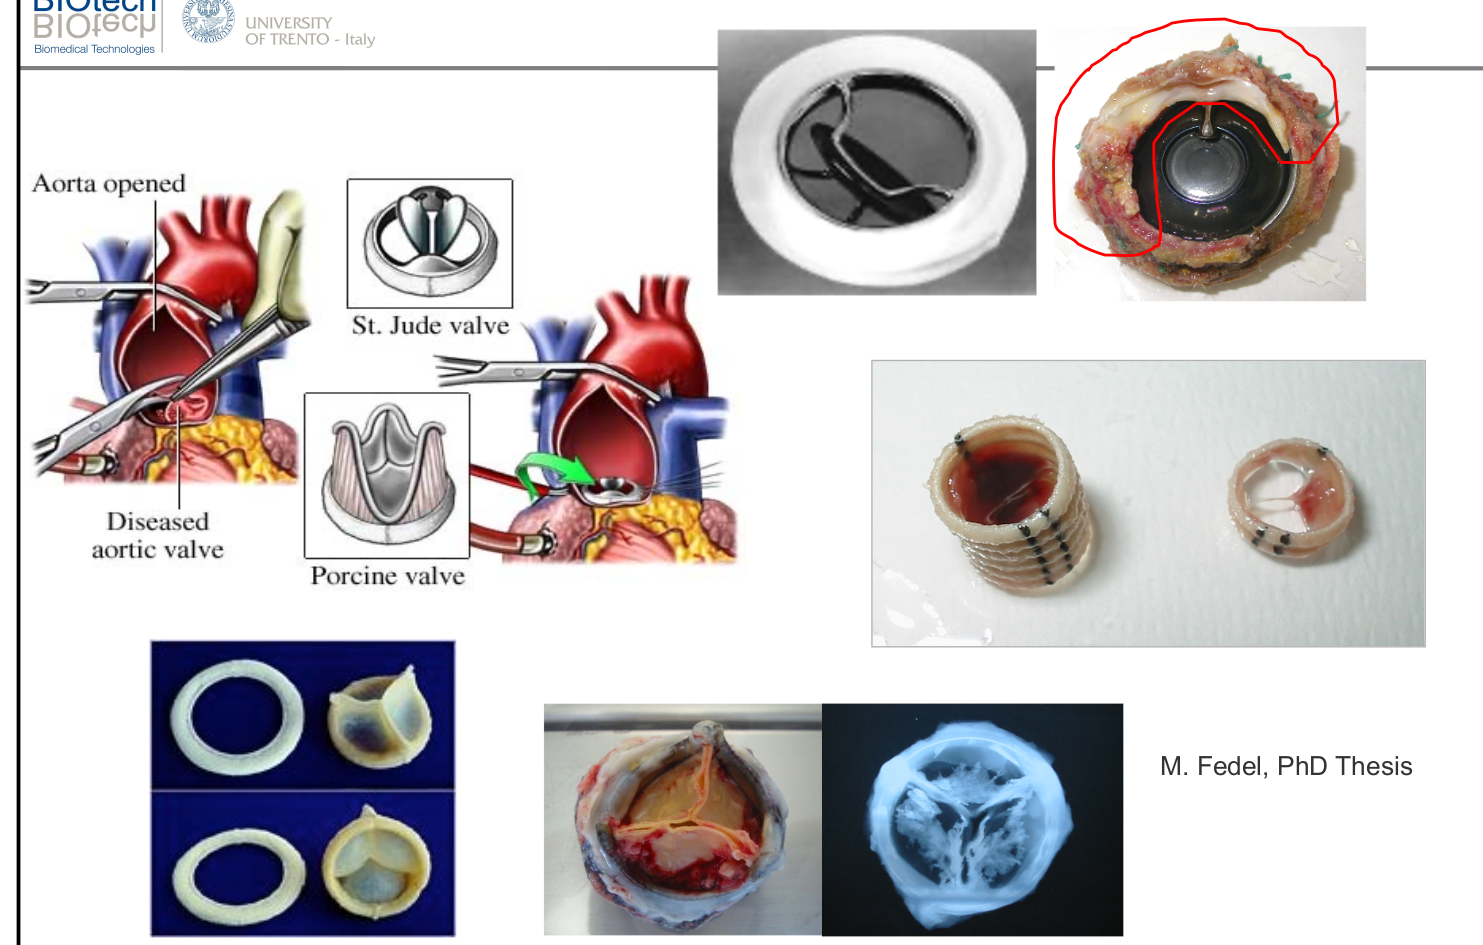
\includegraphics[width=0.5\textwidth]{valves.png}
\caption{\label{fig:valves}}
\end{figure}
	People however changed idea based on what they discovered after seeing what happened in the body after some time after implantation.
	Heart valve made of titanium and polyester failed because around the plastic layer the body built a very thick scar tissue and the valve could not open any more.
	The same valve in another patient induced trombosis.
	This first valve was treated with anticouagulants.
	The context of implantation is extremely important.
	A biological heart valve was harvested from pigs, but it failed because of calcification which rendered the valve unable to close.
	All the material induce a biological reaction.
	No material is completely inert, because our antibodies can recognize anything that is not "self".
	\\
	The concept of biocompatibility was revised: the ability of a material to perform a specific application causing an appropriate host response in a specific application” (1987).
	\\
	\begin{figure}[ht]
\centering
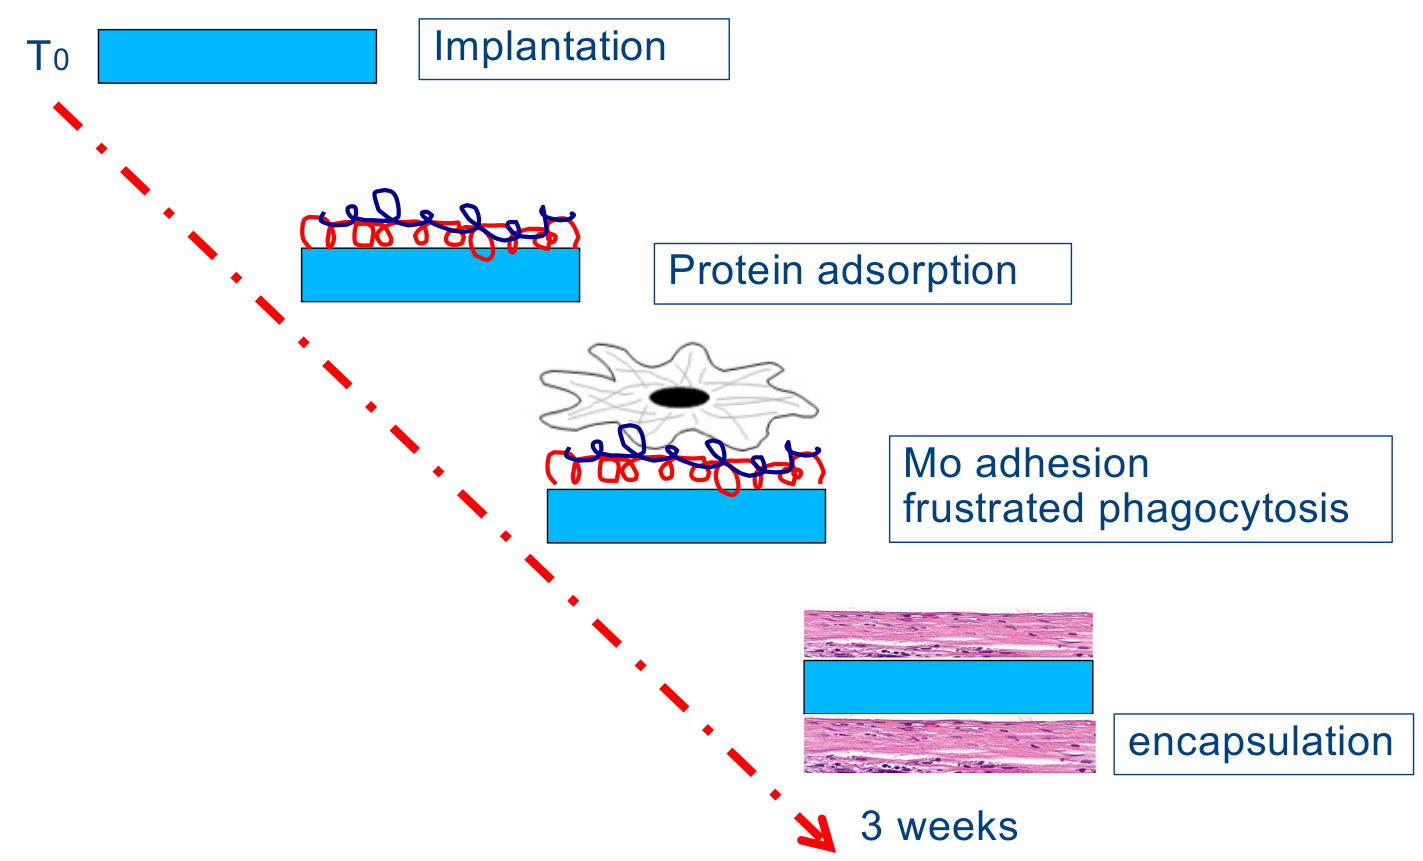
\includegraphics[width=0.5\textwidth]{fbrx.png}
\caption{\label{fig:matrixome}}
\end{figure}
	We can take as an example FBRx (cos'è?????), a non porous scaffold material.
	Depending on the chemistry of the material a specific protein adsorption is activated and subsequently an immune response.
	But if the material is not degradable, the macrophages start to coat the foreign body with scar tissue.
	At this point the reaction is finished.
	If the scaffold degrades eventually we will have an empty bag.
	Just by changing the porosity the scar tissue is reduced and regeneration is promoted.
	\\
	Injectable gels (hydrogel) are useful when filling cavities, becomes scaffold and supply for a scaffold for cells to migrate to.
	\\
	Take home lesson: scaffold should be tissue-organ dependent, defined situation, specifically react with the tissue (induce activation of cellular function to heal in a specific environment), material degradation.

	\subsection{Re-evaluation of the biocompatibility concept}
	Some factors led to the redefinition of the concept of biocompatibiliy, as for the scaffold is not enough to simply "exists":

	\begin{multicols}{2}
		\begin{itemize}
			\item Response to specific materials could vary from one application site to another (tissue-organ dependent) and not just on the material characteristics but it should also defined the situation in which the material is used (pathology, function).
			\item An increasing number of applications require that the material specifically react with the tissues rather than be ignored by them.
				Some applications required that the material degrade over time in the body rather than remain indefinitely.
			\item
		\end{itemize}
	\end{multicols}

	Most advance concept: biocompatibility is not a material's property but a system's property. It cannot be defined without considering the context.

\section{The complexity of the biocompatible system}
\begin{figure}[ht]
\centering
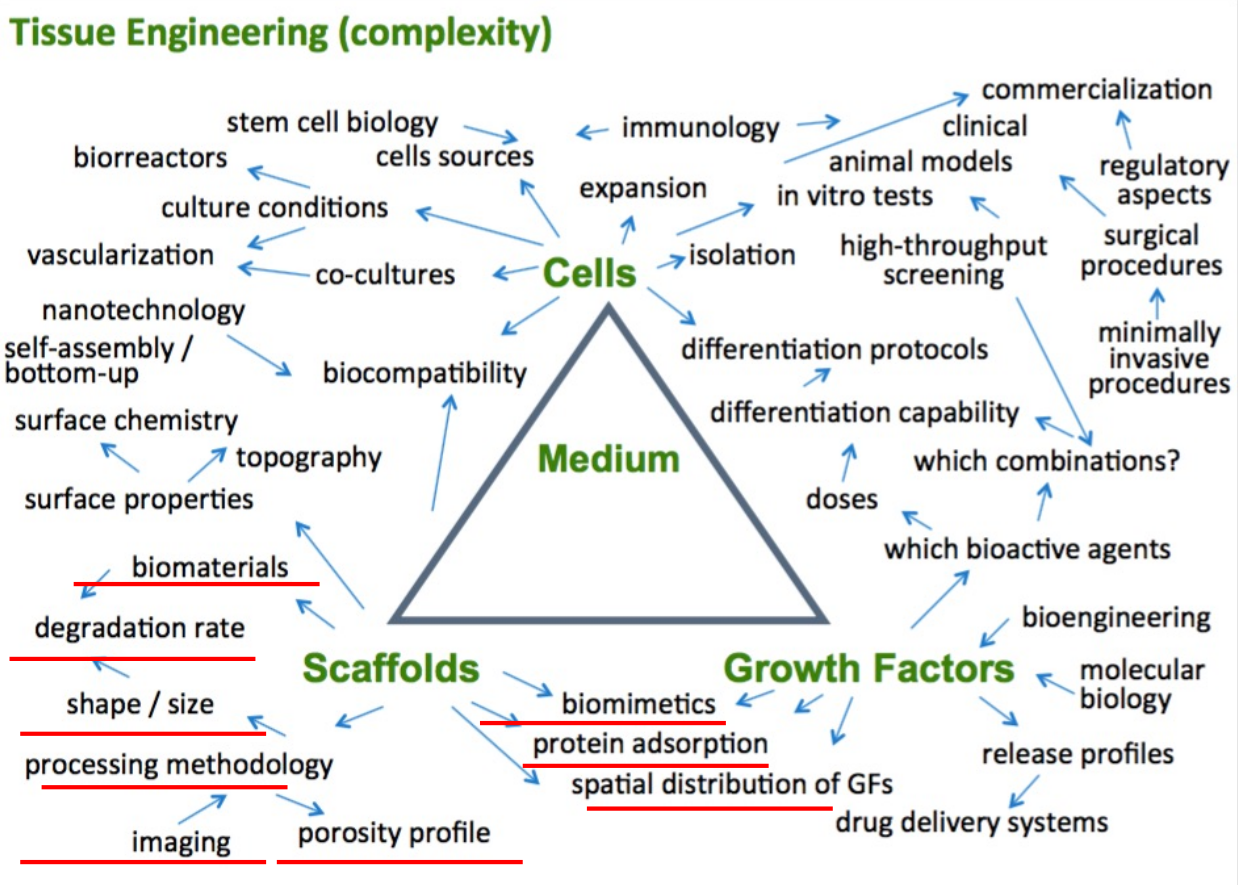
\includegraphics[width=0.8\textwidth]{piramide_completa.png}
\caption{\label{fig:complete_pyramid}}
\end{figure}
Tissue engineering as a triangle: it seems easy with only three actors.
Each one has many possibilities!
\\
For a scaffold to be biocompatible the following steps must be followed:

\begin{multicols}{2}
	\begin{itemize}
		\item Determination of native tissue-organ.
		\item From in vitro to in vivo (from smaller to bigger animals, that depending on the biological problem).
		\item At this point we need to define the surgical model and finally we move to clinical trials.
		\item In addition, for in vitro test now bioreactors are used, because we don't want steady conditions but we want mechanical stimuli (the perfusion provides stress but also washes away cell residues).
	\end{itemize}
\end{multicols}

	\subsection{ECM molecules production: effect of the mechanical stimuli}
	\begin{figure}[ht]
\centering
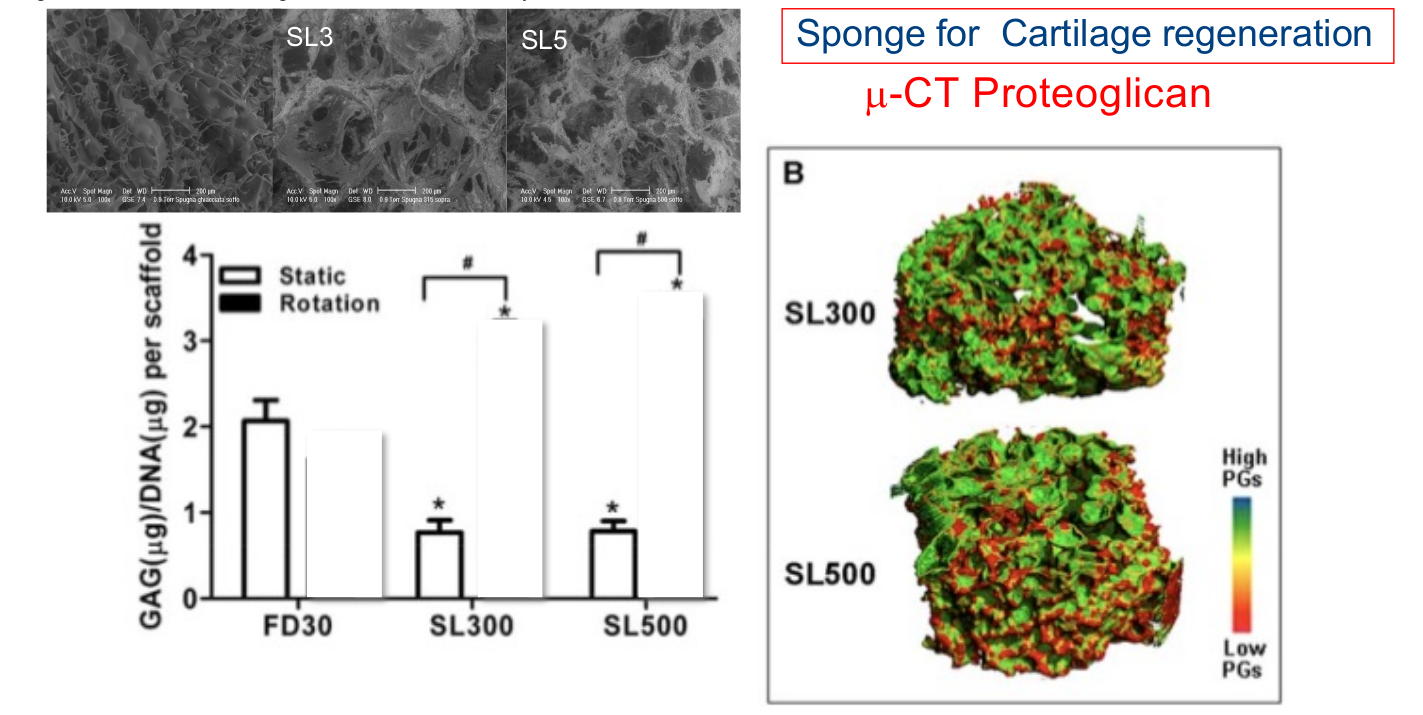
\includegraphics[width=0.5\textwidth]{sponge.png}
\caption{\label{fig:matrixome}}
\end{figure}
	Different sponge-like scaffolds were produced with different properties (like porosity) for cartilage regeneration.
	The quality of GAG (mainly into the ECM of cartilage) was assessed.
	In addition, microCT to see where the GAG is and the sponges are completely infiltrated with it.
	SL500 had a lot of green (GAG) but only on the outside.
	What happens if the devices undergoes a mechanical stress similar to the biological situations? We get the exact contrary! Just by changing from a static to a perfusion situation.
	By changing the environment we ultimately change integrins and biological performances.
	In perfusion, the integrins were upregulated! Integrins are transmembrane proteins: portion inside and outside and are important so that scaffolds are able to talk to cells, instructive behaviour.
	Cells are extremely sensitive.
	In the very first case the in vitro model was not well designed.
	We must perform extensive and well thought tests before moving to the application.

    \graphicspath{{chapters/ecm/}}
\chapter{ECM}

\section{ECM functional role}
The functional role of the extracellular matrix in tissue engineering involves providing a starting point for scaffold biodesign.
The ECM is a dynamic environment, which is produced and regulated by cells.
The ECM performs the following functions:

\begin{multicols}{2}
	\begin{itemize}
		\item aids in cell locomotion: cells in the body are in movement, mediated by the action of receptors (transmembrane proteins) and ligands into the ECM. The ECM should provide ligands for adhesion, which should be patterned in order to direct the cells in a specific place;
		\item transmits and distributes mechanical loads: the ECM, depending on the tissue and mechanical stimuli, should assume a specific structure in order to transmit the stress to the cells, without damaging them.
			Considering the scaffold design, this means that the mechanical properties of the scaffold are really important.
			The best mechanical properties to reproduce depend on the context;
		\item prevents premature mechanical failure;
		\item partitions cells and tissues into functional units;
		\item acts as a scaffold defining tissue and organ architecture;
		\item acts as a storage and dissipative device for elastic energy;
		\item acts as substrate for cell adhesion, growth, and differentiation: cell adhesion is really important, and should be provided even for cell growth and differentiation, because cells are adhesive dependant - especially cells for regeneration. This means that activation requires adhesion.
	\end{itemize}
\end{multicols}

\noindent
The ECM is a controlled complex network. It is formed by a complex network of proteins, glycoproteins and proteoglycans, which together provide tissue specific biophysical and biochemical properties. Remember that the ECM is tissue specific. The contact between the nucleus and the ECM is performed by integrins. We must find which genes should be activated for stimulating regeneration and the ligands for gene activation.
\\
\noindent
The ECM must interact with the cells. If the interaction is interrupted, the cells may go into pathology.
The ECM provides not only mechanical and structural support to cells and tissues, but also binds soluble ligands and transmembrane receptors to provide spatial coordination of signalling processes.
The ability of cells to sense the chemical, mechanical and topographical features of the ECM enables them to integrate complex, multiparametric information into a coherent response to the surrounding microenvironment.
Consequently, dysregulation or mutation of ECM components results in a broad range of pathological conditions.
\\
\noindent
The ECM is a composite material where cells sense the environment.
An example is a chondrocyte in a bone-like environment that will transform into bone, via calcification.
We need to pay attention to not having a damage effect instead of a therapeutic effect.
ECM polymers/network are instructive,  they provide structural and mechanical integrity to tissues.

\section{Components of the ECM}
\begin{itemize}
\item Physical signals are from fibronectin, vitronectin, collagen, laminin, fibrillin, GAGs, PG,...
\item Soluble signals: CF, cytokines, chemokines,...
\item Structure: composites, fiber-based, function dependent
\item Water: used to better tune mechanical properties. It can help the material to support the stress. Water is highly present in articular cartilage! The molecules able to ligate the water are GAGs and PGs. More water means more GAGs and PGs.
\item Mechano-transduction: translating mechanical stimuli
\end{itemize}
\noindent
Fibers are made of collagen, which can form fibrils (very elastic structures), fiber (a little bit thicker) or bundle (composition of more fibers all together). In addition, to better tune the mechanical properties without changing the chemistry, nature can also change the organisation of the fibers: they can be well oriented or randomly distributed, depending on the mechanical stimuli and the direction of them.
\\
\\
\noindent
Signals are important for the adhesion, so other molecules are introduced into the scaffold as well, adhesion ligands and collagen (to form the structure, it is able to provide ligand too).
Another strategy is trying to reduce the number of the elements, in particular the number of the molecules produced by the cells. How? By designing multi-functional polymers, one polymer must do many things. Finally, it is possible to employ soluble signals. Cells can communicate with each other - very distant cells communicate thanks to soluble signals.
\\
\\
\noindent
Thanks to the cross-talk between cells and ECM we have the trigger and the control of many processes. ECM/cells crosstalks facilitate and regulate: pattern formation, morphogenesis, cell fate, daily cellular processes, wound healing, tissue homeostasis.

\subsection{Stem cells}
The environment is important even for stem cells. Stem cells are rare cells that are uniquely capable of both reproducing themselves (self-renewing) and generating the differentiated cell types that are needed to carry out specialised functions in the body.
This is important in the embryogenesis and a balanced control between self-renewed cells and differentiation is fundamental in the healing process and homeostasis. If it is deregulated we can have tumorigenesis, degeneration, pathology,...
Pay attention: the scaffold sends information, we can induce cancer formation too!
Changing the organization of the fibers in the ECM leads to modifications in water content and rigidity ; as a result, we will end up with a completely different signal.

\section{The matrixome: chemistry of the ECM}
\begin{figure}[ht]
\centering
\includegraphics[width=0.8\textwidth]{matrixome}
\caption{\label{fig:matrixome}}
\end{figure}

\noindent
The stiffness is controlled by collagens, elasticity by elastic fibers.
Signalling molecules are used for cell-cell communications e.g. growth factors.
Adhesion molecules promote cell adhesion, pattern to drive the mobility direction.
The proteinases are important to destroy the proteins we don’t want, they provide dynamicity. The GAGs and PGs are relevant for the water content of the ECM.
Something important for scaffold design is that we can use proteinase to degrade the scaffold once we need to degrade it, not before.
\\
\noindent
Matricellular proteins are extracellular modulators of cell function expressed at high level during development and in response to injury. They are modulators of cell matrix interactions and bind to many cell surface receptors, the ECM, GFs, cytokines and proteases. Their role is to induce de-adhesion in contrast to the adhesivity of most matrix proteins (migration).
\noindent
Functions:
\begin{itemize}
\item cell adhesion, migration, chemotaxis
\item matrix assembly and collagen fibrillogenesis
\item regulation proliferation/apoptosis
\item binding/activation GFs and cytokines
\item angiogenesis and tumour growth
\end{itemize}

%Example: support of a state of intermediate adhesion (disruption of focal adhesion and reorganisation of actin stress fibers):	TSP1 and 2, Tenascin-C, SPARC
%Cercare più info/appunti

\section{Collagen}
Collagen is one of the most important proteins for the ECM, as it provides structural properties. Collagen is produced by cells: the production starts in the cytoplasm,  while the final assembly is performed outside the cell.
Fibrils are formed first, then assembled into fibers and bundles.
\noindent
How can collagen build the network?
\begin{itemize}
\item connective tissue: less density, soft network, more water, fiber and fibrils
\item meniscus: parallel fibers, more density, packed fibers, because of different functions, bundle (more stress)
\item myocardium: mechanical stresses, it should support the growth in one direction
\end{itemize}
\noindent
Cells can migrate in this low porosity material through a specific enzymatic process,  which allows the space to be opened up.
Collagen is non-homogeneous, bottom-up, multi-functional, dynamic and has a hierarchical structure. The structure is function dependent.
We have three chains,  which can reach a helix formation (quaternary structure). If we increase the chemical bridges between the helices we control elasticity.
\\
\\
\noindent
The ECM is degraded by cell-secreted proteases (remodelling) and releasing of bioactive component.
Natural ECMs modulate tissue dynamics through their ability to locally bind, store and release soluble bioactive ECM effectors such as GFs.
Our scaffold should promote cell migration.
\\
\\
\noindent
Collagen is a family of proteins, we have at least 23 different types of collagens. Depending on the tissue, we have the prevalence of one type on another type. In the cartilage for example we have collagen type II. In tendons we have type III collagen, which is really similar to jellyfish collagen, currently commercialized.

\section{Fibronectin}
Fibronectin is a large matrix glycoprotein present in most body tissues fluids.
Functionally, it is the classic example of an adhesive glycoprotein, binding and interconnecting extracellular matrix components with each other and to the surface of the cells.
It is one of the most important molecules through which cells interact with the surrounding environment.
The binding of fibronectin to the cell surface’s integrin receptors plays a critical role in the cell migration (during the development and postnatally).
\\
\\
\noindent
Fibronectin is made of two identical chains connected by a disulphide bond, a dimer.
We can recognise different sections:
\begin{itemize}
\item one can interact with fibrin and heparin
\item one can interact with gelatine and collagen
\item one can interact with the cell receptor (arg-gly-asp ac. sequence)
\item one can interact with polysaccharide heparin
\item one can interact with fibrin
\end{itemize}
\noindent
These molecules must be able to interact and crosslink because in this way if we have a stimulus that acts in the collagen, for example, the other parts of the ECM can sense said stimulus. In addition, many regions of the ECM are able to interact with cells, controlling the structure and cellular activity.
\\
\\
\noindent
In ECM we have fibronectins, collagen, gel-forming polysaccharides, water, actin and the cell (figure \ref{fig:structure}).
The transmembrane can sense what is going on in the external side and transfer the information to the internal part and eventually to the nucleus to activate a specific gene expression.
The interactions are important and interesting, the scaffold needs to provide the ability to interact with the same exact mechanism and cells must work in an appropriate way.
We don’t want dysregulation of the mechanisms and the tissue, so we need the natural mechanism of interaction.

\begin{figure}[ht]
\centering
\includegraphics[width=0.6\textwidth]{structure}
\caption{\label{fig:structure}}
\end{figure}

\noindent
The ECM is a mosaic structure, a guide for cell functions.
Should the scaffold replicate the ECM? Partially, yes, but especially the functions!
Large molecules are difficult to manage, maybe using a smaller molecule (nectin instead of fibronectin) is easier.
Fibronectin is needed to reproduce the complete ECM, but nectin is sufficient to promote cell growth.

\subsection{Fibronectin multifunctionality}
The RGD-loop is strategically placed to undergo strong conformational changes and constitutes a mechanosensitive switch for recognition by integrin receptors.
Depending on the mechanical stimulus, fibronectin can assume specific conformations, changing its activity.

\section{Proteoglycans and GAGs}

\textbf{Proteoglycan}: head core protein + chain of polysaccharides (GAGs), which is hydrophilic (figure \ref{fig:pgag}).
Proteoglycans are responsible for controlling the water content of the tissue and are especially important in case of mechanical stresses.
Many proteoglycans can be linked together via long hyaluronic acid chains, forming giant com- plexes.
Because of their negative charges, glycosaminoglycans and proteoglycans together control the $H_2O$ content of the tissue, determining the degree of ”squishiness” of the matrix.
They also allow for $H_2O$ reentry after tissue compression: in this situation water gets squeezed out and the negative charges of different molecules draw near.
This generates an electrical repulsion that summons water from the peripheries.
\\
\\
\noindent
\textbf{Glycosaminoglycans} (GAGs) are linked to the core proteins, we can have:
\begin{itemize}
\item hyaluronic acid
\item chondroitin sulfate
\item keratan sulfate
\end{itemize}
\noindent
GAGs are long linear polysaccharides consisting of repeating disaccharide units (i.e. two-sugar units).
The repeating two-sugar unit consists of a uronic sugar and an amino sugar, which is usually sulfated.
\\
\\
\noindent
In proteoglycans, the big protein is able to interact with water and the core protein, hydrophobic, is covered by hydrophilic molecules.
The water should be able to go out when the tissue undergoes mechanical stress to ensure homeostasis.
This is a reversible mechanism,  the scaffold must have specific properties to resist stress and control water flow.
\begin{figure}[ht]
\centering
\includegraphics[width=0.3\textwidth]{pgag}
\caption{\label{fig:pgag}}
\end{figure}

\section{Modelling nature}
Our goal is to stimulate the cell.
The environment is dynamic, and the interactions are possible thanks to the water.
The interactions between cells and environment are relevant to regulate a lot of processes, from cell fate to tissue formation and regeneration.
Our scaffold will be one of the components that will collaborate to regenerate the tissue.
Once again, we need a model, which is nature.
We need to leave cells work in a natural way.
Living organisms naturally provide a multiplicity of materials, architectures, systems and functions, all resulting in from stringent selection process (evolution).
\noindent
Strategy:
\begin{itemize}
\item polymers (materials) able to integrate
\item molecular synthesis (by cells) at very high level of organisation (molecular recognition, multifunctionality, self-diagnostic, destruction-recycling, bottom-up approach)
\item structure (self-assembling, molecule interactions, interfaces, etc) dynamics
(responsive polymers, adaptation, self-healing)
\end{itemize}
\noindent
The bottom-up approach is more bio-mimetic,  as it reflects how nature works [self-assembling blocks, proteins are formed automatically from amino acids].
We should also focus our attention on building a context-specific microenvironment.
\\
\\
\noindent
Apoptosis is a programmed cell death, in which cells are encapsulated by vesicles and removed.
Necrosis instead happens when the cellular membrane is damaged, we have inflammation.
During necrosis the activity of macrophages is increased, producing also inflammation for neighbouring cells.
It has been suggested to induce tumour cell death through apoptosis to avoid upregulating inflammation.

    \input{chapters/05_inflammation}
    \input{chapters/06_biorecognition}
    \chapter{Hydrogels}
Hydrogels were the first biomaterials rationally designed for human use, especially for soft tissue engineering. 
They are a particular class of materials, exhibiting both solid-like and liquid-like properties, consisting of hydrophilic polymer chains and water, that occupies the interstitial spaces (pores) that are defined in the 3D network constituted by the cross-linked polymeric chains. 
\\
\\
\noindent
Water is the major constituent of hydrogels and could reach more than 90 percent of the weigh of the material - although its quantity is dependent on the degree of hydrophilicity of the polymer chains. 
Cells can be added inside the hydrogel before or after gelation. 
In the first case, one must make sure that the gelation itself won’t damage the cells. 
In the second case, porosity must allow for uniform cellular colonization. 
\\
\\
\noindent
Hydrogels’ characteristics can be modulated according to three main variables:
\begin{itemize}
\item Chain composition: they can be natural (usually polysaccharides) or synthetic polymers. The main subvariables are chain length, degree of hydrophilicity and presence of ligands recognizable by cellular receptors (hydrogels must be biorecognizable). The utility of synthetic polymers is that they can be functionalized with these kinds of ligands to allow cell adhesion, but degradability will become a problem.
\item Cross-linking nature: strategy employed to connect the polymeric chains. This act is also called gelation. This could be:
	\begin{itemize}
	\item Chemical crosslinking: the polymer chains are covalently linked. 
This linkage can be obtained in an enzymatic way (if enzymes capable of interacting with the chosen polymers exist). 
The enzymatic crosslinking is also useful because it guarantees the degradability of the scaffold via host enzymes or in a non - enzymatic way, exploiting specific reactions that may require specific reagents.
	\item Physical crosslinking: the polymer chains are held together by molecular entanglements (temporary spatial constraints) and/or secondary forces such as ionic, hydrophobic, and hydrogen bonds. Chemically crosslinked hydrogels always present some degree of physical interaction as well, but the contrary, of course, does not occur. 
Physical crosslinking can be obtained via thermal treatment, pH changes and treatment with organic solvents.
	\end{itemize}
\item Network nature: it’s the overall 3D structure defined by the crosslinked polymers. 
Its main characteristic is the number and the dimension of the interstitial spaces (pores), influenced by polymer chains length and by the number of crosslinkings. 
Pores number and dimension, together with the degree of hydrophilicity of the polymer chains, will determine the maximum amount of water hosted by the hydrogel. 
This in turn will impact the swelling capacity, one of the main characteristics of these kinds of scaffolds.
\end{itemize}
\noindent
Hydrogels can also be designed with the only goal of carrying modded cells to a particular region of the body: in that case non biocompatible, non biorecognizable synthetic polymers can be used to avoid premature hydrogel degradation and unwanted interaction with the cargo and to carry the cells to the targeted location.
\\
\\
\noindent
Hydrogels can also be used to design drug releasing systems: they can function as surrogate matrices to carry modified cells producing a specific therapeutic agent. 
In order to protect these cells from the host’s immune system, the hydrogel itself must be coated by a semipermeable membrane, that must allow the entrance of nutrients and growth factors in the hydrogel and the exiting of the therapeutic products.

    \graphicspath{{chapters/scarring/}}
\chapter{Fetal healing}

\section{Scarring}
A scar is a densely packed disorganized collagen bundle, with absence of hair follicles, sebaceous glands and other appendages. 
Scarring and fibrosis dominate some diseases in every branch of medicine and surgery.
Examples: skin incisions heal with scars (pathological processes as keloids, hypertrophic scars, …).

\subsection{Adult scarring}
The mechanism of scar formation involves inflammation, fibroplasia, formation of granulation tissue, and scar maturation.  The acute inflammatory response (pro inflammatory mediators) is followed by the proliferation of fibroblasts, which are cells responsible for synthesizing various tissue components, including collagen and fibrin. During the acute inflammatory phase, circulating progenitor cells migrate to injured tissue. Rapid cellular proliferation occurs, which ultimately results in the formation of new blood vessels and epithelium. Fibroblasts then differentiate into myofibroblasts, which are the cells responsible for collagen deposition and wound contraction. Scar formation ultimately results from excess accumulation of an unorganized extracellular matrix. Although scar remodeling occurs for months to years after the initial injury, complete restoration of the normal extracellular matrix architecture is never achieved. 

\section{Embryonic healing}
In contrast to adult wounds, early gestation fetal skin wounds repair rapidly and in the absence of scar formation. 
The fetus is able to regenerate tissues by assembling collagen fiber in a well organised structure.
The biology of fetal repair must be understood; in particular, cellular and matrix events may provide insights to help to modulate adult wound repair to become more fetal-like.

\subsection{Fetal extracellular matrix}

We should try to mimic the embryonic development procedure, where the ECM is elaborated in parallel with cell differentiation and growth.
In particular, our aim is not to obtain a normal ECM analogue (mature scaffold), but a wound bed matrix analogue suitable for regeneration.
Collagen represents a "mature" scaffold, forming a microenvironment suitable for fully differentiated cells.  If we build a scaffold based on collagen type I, cells which don't usually reside in an ECM made extensively of collagen type I will not interact with the surface, leading to a pathologic response. Example: chondrocytes usually interact with collagen type II, so if collagen type I is present cells will form fibrocartilage. 
\\
\\
\noindent
The fetal extracellular matrix is optimized to facilitate cellular migration and proliferation, which may have important implications in wound healing.
\begin{itemize}
\item collagen content: high content of collagen type II and V, increased collagen synthesis. 
\item hyaluronic acid: in scarless fetal wounds, the hyaluronic acid content of the extracellular matrix is increased more rapidly than in adult wounds, major component.
\item adhesion proteins: scarless fetal wounds have an enhanced ability to up-regulate extracellular matrix adhesion proteins, such as tenascin and fibronectin
\item ECM modulators: fibromodulin inactivates transforming growth factor (TGF)-beta, a key cytokine involved in wound healing, and has been shown to have an antiscarring effect during wound repair.
\item non-sulfonated GAGs
\end{itemize}

\subsection{Fetal mediators of scarless repair}
\begin{itemize}
\item lack of inflammation: decreased platelet degranulation and aggregation,  anti-inflammatory cytokines
\item fibrobrlast cells with high migration rate (affecting collagen depth and cross linking)
\item increased number of HA receptors
\item myofriboblasts appear earlier and then disappear
\end{itemize}

\begin{figure}[h]
\centering
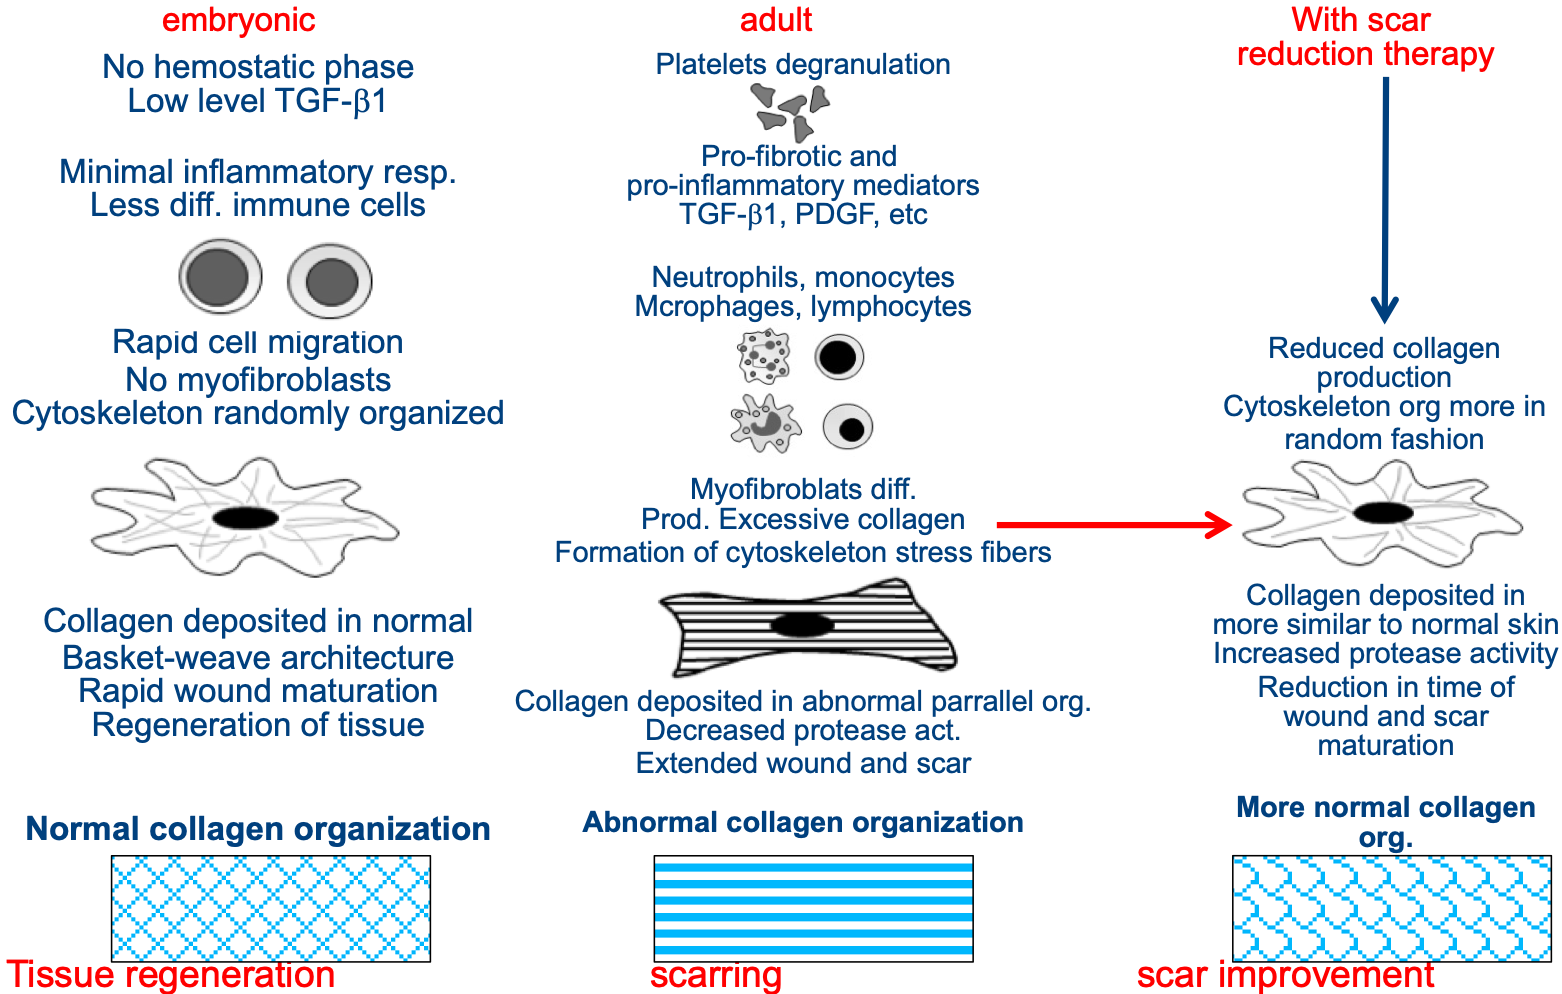
\includegraphics[width=0.5\textwidth]{scar.png}
\caption{\label{fig:scar}A lesson from fetal healing: scarless regeneration}
\end{figure}

\section{Hyaluronan}
Hyaluronan is a hydrated gelatinous material	synthesized from basal side of an epithelial sheet. 
It creates a cell-free space into which cells can proliferate and migrate, perform the diffusion of nutrients, metabolites,...
It is able to resist compressive forces and acts as space filling material in embryogenesis.
It is degraded by hyaluronidase.
\\
\\
\noindent
Hyaluronian is composed by the simplest GAG with a very long chain length (25000 disaccharide units. It lacks sulfated sugars and is usually not attached to protein (used as filler). The high negative charges on the glucuronic acid attract Na+ ions and water.
 
%\section{Collagen assembly}
%Collagen type III is involved in structural maintenance in expansible organs e.g. smooth muscle, blood vessels, connective tissue. Collagen type V instead is responsible for fibril formation in skin, bones and fibrocartilage. In particular,  collagen fibrils have a high content of collagen type III and IV.

\section{Biology of regeneration}
Regeneration of amputated limb can occur at an adult stage in amphibians and fish.
This complex process is enabled by specific tissue regeneration mechanisms.
For instance,  in adults of Homo Sapiens the liver regenerates spontaneously. 
Furthermore, we have little capacity to regenerate tendons and ligaments. 
 


    \graphicspath{{chapters/scaffold/}}
\chapter{Scaffold design}

The dynamics of regeneration vary from tissue to tissue according to the hierarchy of tissue or organ function. 
Remember that “the ability of a material to perform with an appropriate host response in a specific application”.
Important consideration for the materials: 
\begin{itemize}
\item sourcing of functional cells: if the scaffold requires a pre-loading of cells, we need to discuss which kind of cells to employ beforehand e.g. stem cells, cells from the patient (bone marrow, amniotic liquid, etc)
\item GF regulatory systems: synthetic polymers with no biorecognition properties require functionalization
\item immuno acceptance: e.g. force stem cells to become osteoblasts or modulate the immune response in order to shorten the inflammation and boost regeneration
\end{itemize}
\noindent
Biological information is required for performing in vitro tests and for functionalization (linked to specific biological pathways, essential to thoroughly describe the mechanisms).
\\
\\
\noindent
Scaffolds can be grouped in two categories:
\begin{itemize}
\item conductive: provide and maintain a 3D environment that supports a passive cell infiltration, creating a pseudo micro environment. The limitation is that they are not able to provide enough info to promote full regeneration in most applications.
\item  inductive: designed toclosely mimic the native cellular environment and may contain bioactive molecules and naturally or synthetic analogues of structural, functional or specialised proteins and proteoglycans. They can increase the biocomplexity of the system.
\end{itemize}
\noindent
A scaffold is part of a complex system. It is used to direct, by control of interactions with components of living systems, the course of any therapeutic or diagnostic procedure.
A scaffold is composed by different materials e.g. natural and synthetic polymers. 
The geometry should be suitable for the specific application e.g. allow migration, cell distribution in 3D in functional manner, alignment. 
Polymers can be combined with other materials or drugs.
If the interaction and biocompatibility are present, we will have a suitable response.

\subsection{Tissue engineering strategies}
\begin{itemize}
\item "just" scaffold in vivo: the body helps with the regeneration, if possible it’s the best strategy we can follow.
\item scaffold + cells implantation: we need to define why we wish to culture in vivo e.g. ECM production, differentiation,…
\item cell sheet engineering: fabrication with cells (stem cells) from the patient. 
\end{itemize}
\noindent
Cell sheet engineering is the only bottom-up approach, starting from the material and not the biology. 
%Thermo responsive polymers: different orientations and activity depending on the temperature while lamina: thermo responsive polymers, culture at 37° C → laminar produced after this procedure.

\subsection{Biocompatibility requirements}
Revised performance criteria for the 4th generation of biomaterials:
\begin{itemize}
\item tailored biodegradation
\item amenability to engineering design and manufacturing
\item induces cell and tissue integration
\item smart (i.e. physiologically responsive)
\item instructional (i.e. controls cell fate)
\item mechanical strength and function (i.e. mechanical signalling)
\end{itemize}

\begin{figure}[h]
\centering
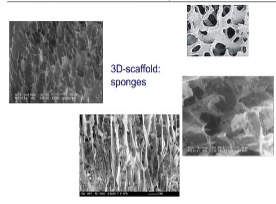
\includegraphics[width=0.5\textwidth]{sponge.jpg}
\caption{\label{fig:sponge}}
\end{figure}
\noindent
Fig \ref{fig:sponge} repair of trabecular bone with 3D-scaffold sponges. 
All of them are artificial scaffolds, while on the top right we have the natural sponge. 
The porosity can be oriented or random, with different geometries.
The scaffold should promote adhesion, proliferation and migration. Hypoxia should be avoided, maybe with early angiogenesis. 
In vivo: in the case of bones, we have osteoblasts adhesion and migration, ECM production. In order to avoid hypoxia and necrotic tissue formation it is required to achieve vascularization, we need to supply oxygen to stimulate angiogenesis. 
In vitro: millimetres not microns, the problem is more tough. We could culture in a bioreactor e.g. chamber with medium forced to go through, or include into the scaffold oxygen donors.

\subsection{Experimental data discussion}
\begin{figure}[h]
\centering
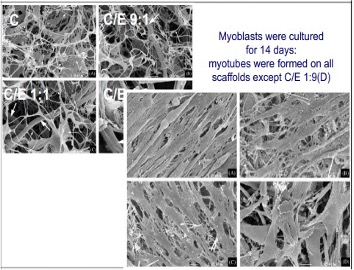
\includegraphics[width=0.5\textwidth]{myoblast.jpg}
\caption{\label{fig:myoblast}}
\end{figure}
\noindent
Fig \ref{fig:myoblast}: muscle regeneration. Use collagen, elastin and glycosaminoglycans. GAGs control water content and mechanical properties. Elastin is required for muscle elasticity, collagen for the strength.
It is necessary to find the optimal ratio among the components.
By changing the ratio,  we have 4 different architectures:
\begin{enumerate}
\item C: sponge, similar to natural behaviour of collagen
\item C/E 9:1: the big fiber starts to appear (elastin)
\item C/E 1:1: similar content
\item C/E 1:9: a lot of big fibers pink fiber: elastin fiber
\end{enumerate}
\noindent
C might not be optimal, as well as C/E 1:9, as they are quite different from biological setting.
In vitro test: after two weeks myoblasts were cultured for 14 days and myotubes were formed on all scaffolds except C/E 1:9(D).  We witness a different organisation of the myotubes; in the last example, myoblasts are not able to organise as the condition is very far from physiology.
By considering the test, the best samples seem to be C/E 9:1 and C/E 1:1 .
\\
\\
\noindent
Tissue engineering is 3D assembly over time of vital tissues-organs by a process involving cells, signals, and the extracellular matrix.
\begin{figure}[h]
\centering
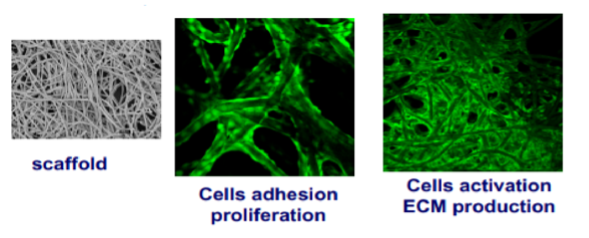
\includegraphics[width=0.6\textwidth]{3D.png}
\caption{\label{fig:3D}}
\end{figure}
In this case we have a scaffold for bone regeneration and osteoblast proliferation (fig \ref{fig:3D}).  The cells (green) are able to adhere, proliferate and migrate. The scaffold is then completely covered in cells. We then witness tissue-specific ECM production, mineralzation. This is a great starting point, but we have to better understand the degradation process of the scaffold and also vascularisation!
How can we check in vivo vascularisation? We need to perform co-culture of osteoblasts (angiogenesis factors + collagenic structure for capillary network formation) and endothelial cells (use empty spaces to assemble as a tube). To obtain a physiological situation we need a careful design.

\section{Scaffold examples}
\subsection{Example 1}
\begin{figure}[h]
\centering
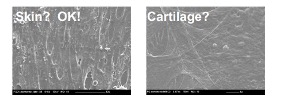
\includegraphics[width=0.6\textwidth]{sk_car.jpg}
\caption{\label{fig:sk_car}}
\end{figure}
Fig \ref{fig:sk_car}: film with same polymers, same architecture, different cells: keratinocytes and chondrocytes. The two films were completely spread.
Cells grown in a flat dish tend to behave as individual cells or forming a monolayer, whereas cells cultured in a 3D space are more likely to assume the characteristics of a particular tissue. 
Cartilage, once grown flat, is almost impossible to shape into joints. The scaffold here, in the case of cartilage, is inducing the loss of the original phenotype,  so it is not biocompatible.
In the case of the skin, it is promising for biocompatibility, very compact and well connected monolayers.

\subsection{Example 2}
\begin{figure}[h]
\centering
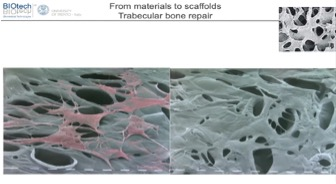
\includegraphics[width=0.5\textwidth]{bone.jpg}
\caption{\label{fig:bone}}
\end{figure}
Fig \ref{fig:bone}: in this case we do not have biocompatibility at all. The cells adhere to the polymer but do not migrate, so we should increase the porosity. 
After few days: we have a multi-layer as result, no migration and no biocompatibility. 

\subsection{Example 3}
\begin{figure}[h]
\centering
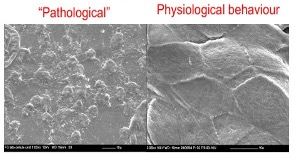
\includegraphics[width=0.5\textwidth]{suine.jpg}
\caption{\label{fig:suine}}
\end{figure}
Fig \ref{fig:suine} suine primary urothelial cells, 6 days after seeding. 
The right image has the geometrical shape of the cells, the phenotype is ok. 
Left: cells don’t connect and are disorganised, so they do not communicate. 
They are more round shaped, so the adherence is not good, there is no activation.

\subsection{Example 4}
\begin{figure}[h]
\centering
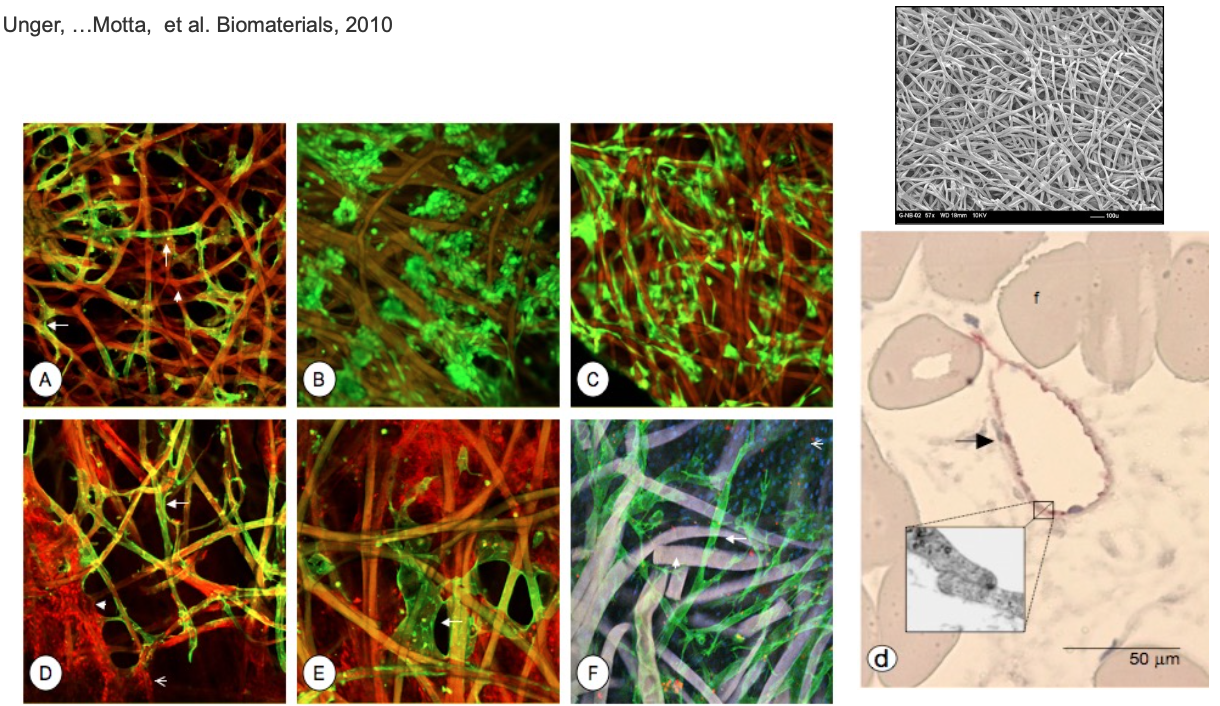
\includegraphics[width=0.5\textwidth]{fibroin}
\caption{\label{fig:fibroin}}
\end{figure}
Fibroin micronet (Fig \ref{fig:fibroin}) human microcapillary endothelial cells (HDMEC) and primary human osteoblast cells (HOS) in coculture (10 days). Very good results, empty tubes, but it is promising. They can be put into the scaffold and then maybe used as vessels. Issue: We have to pay attention if the vessels connect to our circulatory system!

\subsection{Example 5}
\begin{figure}[h]
\centering
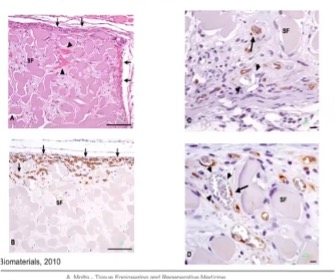
\includegraphics[width=0.5\textwidth]{osteoblast}
\caption{\label{fig:osteoblast}}
\end{figure}
Figure \ref{fig:osteoblast}: pre-vascularized fibroin net, in vivo anastomosis with host vasculature.
Brown tubes: in vivo, blood cells are present and anastomise. 
Left: loaded with osteoblast, let grow and then implanted. Fast angiogenesis, not too many vessels, only in the surface
Right: loaded with osteoblast, immediately implanted.
In vitro human cells and implanted in rat to identify the difference. On the right there are some capillaries that were produced and there is not red blood cells.

\subsection{Example 6}
\begin{figure}[h]
\centering
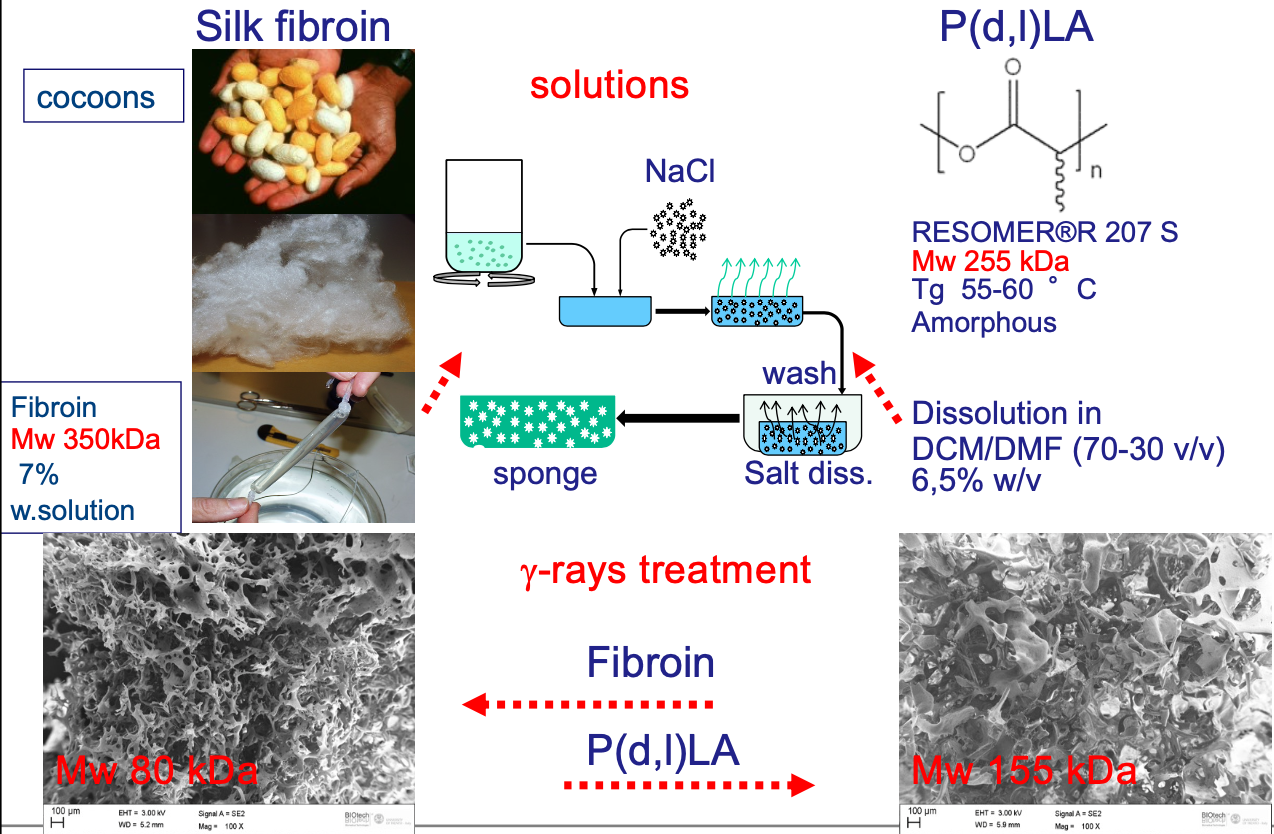
\includegraphics[width=0.5\textwidth]{salt}
\caption{\label{fig:salt}}
\end{figure}
Figure \ref{fig:salt}: from a NaCl solution salt crystals will form a sponge. The porosity depends on crystal size. We can then apply gamma rays treatment and add either silk fibroin or P(d,l)LA.

MISSING LECTURE

\section{Cell encapsulation}

The cell encapsulation methods consists in the entrapment of cells in microcapsules or microbeads starting from a suspension of cells in polymeric solution that can be solidified by chemical or physical methods. 

\section{Electro-hydrodynamic jetting (EHDJ)}

In the electro-hydrodynamic systems a solution is fed through a positively charged metallic needle. The solution reacts to the presence of the charge, generating repulsive coulombic forces on its surfaces, causing the deformation of the meniscus at the tip of the needle into a Taylor cone. If the voltage is high enough, the electrostatic repulsion on the surface can overcome the surface tension at the apex of the liquid cone, leading to its disintegration (Rayleigh limit) and creating a jet of drops.
There are some parameters that we have to assess:

\begin{multicols}{2}
    \begin{itemize}
        \item Speed;
        \item Starting concentration of cells;
        \item Starting concentration of polymer;    
        \item Type of polymer. 
    \end{itemize}
\end{multicols}

Taking in consideration these parameters we are able to control the final number outside of cells onto the beads. We can also check the quality of the concentration using a confocal microscope with live/dead staining. With this process is possible to check how many cells are alive and assess an optimal number of cells. 

    \subsection{Cell encapuslation requirements}
    
    \begin{multicols}{2}
        \begin{itemize}
            \item The encapsulation material (polymer should permit the free passage of nutrients and oxygen (in) and waste products (out) as well as of therapeutic protein products.
            \item Encapsulation material should prevent high Mw molecules, antibodies and other immunogenic moieties from contacting the encapsulated cells. 
            \item The encapsulation material should protect cells from mechanical stresses and from the host's immune-response.
            \item The encapsulation material and method should not damage cells neither affect their behavior, as related to the desired function/application.
        \end{itemize}
    \end{multicols}
    
    \subsection{Cell encapuslation applications}
    Possible applications for cells encapsulation are drug delivery, bioartifical organs and tissue engineering. 
    
    \begin{multicols}{2}
        \begin{itemize}
            \item The encapsulation of therapeutic cells permits the implantation of allogenic and xenogenic cells for the regulation of certain physiological processes damaged by death or senescence of host tissues. 
            \item Microcapsules injected at the transplantation bed allow the release of biomolecules produced by the encapsulated cells, such as insulin produced by encapsulated beta-cells for diabetes type I therapy, pro-angiogenic or anti-angiogenic growth factors to enhance or inhibit vascularization.
            \item Microencapsulated cells can be used as building blocks for the fabrication of tissues/tissue precursor in vitro or implanted in vivo for tissue regeneration.
        \end{itemize}   
    \end{multicols}

\section{Organ Printing - Bioprinting}

\section{Short-term encapsulation effect}

\begin{multicols}{2}
    \begin{itemize}
        \item The main function of HSP proteins consist in cells protection against apoptosis, necrosis, hypoxia or any other type of stress.
        \item Elevated co-erexpression of HSP70B' and caspase-3 genes points to mild stress conditions, and cells protection activity.
        \item The results were supported with Live/Dead test, where we can observed cell death within 48 hours after encapsulation
    \end{itemize}
\end{multicols}



    \graphicspath{{chapters/vascularization/}}
\chapter{Vascularization}

\section{Angiogenesis and pore size}
Angiogenesis is the bottleneck of tissue engineering. 
In order to regenerate functional tissues, stimulation and control or inhibition of angiogenesis are critical.
The porosity of the scaffold is fundamental for promoting vascularization.
A broad distribution of pore sizes and pore shapes ranging from very small to very large can be required.
\\
\\
\noindent
In fig \ref{fig:pores} we have the design of a very simple porous scaffold. 
Building technique: combine the polymers with spheres, with holes filled with water and then emptied. 
The ratio between spheres and solution has to be tuned carefully.
Black holes are interconnections. Another technique is salt leaching, where we first add crystals to polymeric solution and then salt is removed.  The regular shape is kept fixed thanks to crystal. 
In the case of spherical pores,  the interconnection depends on the number of spheres per volume. We can modulate size and interconnection by selecting the concentration. 

\begin{figure}[h]
\centering
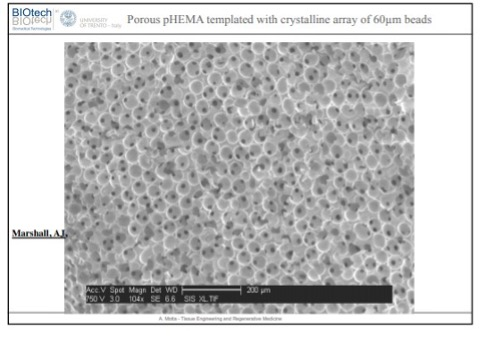
\includegraphics[width=0.5\textwidth]{pores}
\caption{\label{fig:pores}}
\end{figure}

If we analyze an image at higher magnification,  we observe that black dots measure around 5 micron. 
By playing with the scaffold, different families can be obtained. 
Results: more capillaries in the case of smaller pores. Ideal range: 40-50 microns. 
The highest vascular density was observed in the case of smaller porosity (0-100 micrometers). 
The range was explored in depth, 20 micron something appeared, the highest is around 40 micron. Very large porosity leads to the formation of a layer of endothelial cell, no 3D tube required for vascularization.  

\section{Scaffold vascularization strategies}
\begin{enumerate}
\item growth factor delivery: delivery of single or multiple angiogenic GF to stimulate. loading molecules can be performed by mixing with the polymer (fast release), include them in a drug releasing system (polymeric nanoparticle, driven by degradation time of nanoparticles ) or link the molecules to the polymeric chain. Which is the rational of the choice? It mainly depends on required timing. Strategies can be also combined in order to release our molecule at different times.
\item cell transplantation: implant EC on the tissue
\item in situ vascularisation with endogenous cells
\item scaffold pre-vascularization: pay attention to the protocol used. We must be sure that robust tubes tar produced in order to anastomize with the osteoblasts. We can also include something to attract already existing vascular tubes to the scaffold.
\item decellularised scaffold: decellularised myocardium, not populated by endothelial cells. We take a piece of myocardium, decellularize but leave the basic structure, including tube. The main difficulty in this strategy is to guarantee a very low amount of DNA (check that no debris is left after decellularization), avoid thrombogenesis through forced migration to reform endothelium.
\item angiogenic biomaterials: the best option if possible, design biomaterials able to induce vascularization per se. We can call them “precision biomaterials”, as they are designed according to have a specific function. Nature derived biomaterial: e.g. protein derived from silk, intrinsic angiogenic potential. Synthetic functionalized biomaterials.
\item microfabrication methods: top-down approach, answer to build up vessels and around them the tissue. We can bypass the issue of decellularize by directly inserting endothelial cells.
\end{enumerate}

\section{Angiogenic potential evaluations}
In vitro procedures should be carefully designed, we need to make sure that we are obtaining useful considerations on the scaffold. 
Fig \ref{fig:coculture} : seed mononuclear cells inside the hydrogel upon isolation of two main endothelial progenitor cells populations from peripheral blood.
Impact on the matrix: cells were seeded and checked after 4 and 10 days. In the case of IKVAV modified culture we have more signals. This means we have more cells, more clusters and more layers (migration). The aim was to design a precision material to be used in brain, laminin derived (brain ECM). Strategy:  isolate peptide involved in differentiation and link it to polymeric chain. 
We expect to obtain tubes in angiogenesis, but here we only observe a bunch of cells. What was wrong is the in vitro model, too far from physiology because only one layer is not good. The model was then changed: in order to reach a tube more cells are required e.g. cells able to drive tube formation -> bone marrow stem cells, which differentiate into pericytes, secrete angiogenic factors e.g. VEGF and Ang-1 and produce collagen I and IV for the ECM. 
\\
\\
\noindent
For stem cells isolated from donors we need to at least use 5 replicates, as there is a huge variability.  By applying this procedure, we can see a nice formation of tubes (well branched and interconnected) in donor 1, only pieces in donor2 and 3. Takehome message: take into consideration personalized solution in order to avoid variability and to achieve the best result. Secondly the result in co-culture was identical in terms of ECM. If the culturing conditions are good and we introduce SC, we can successfully reach vascularization.

\begin{figure}[h]
\centering
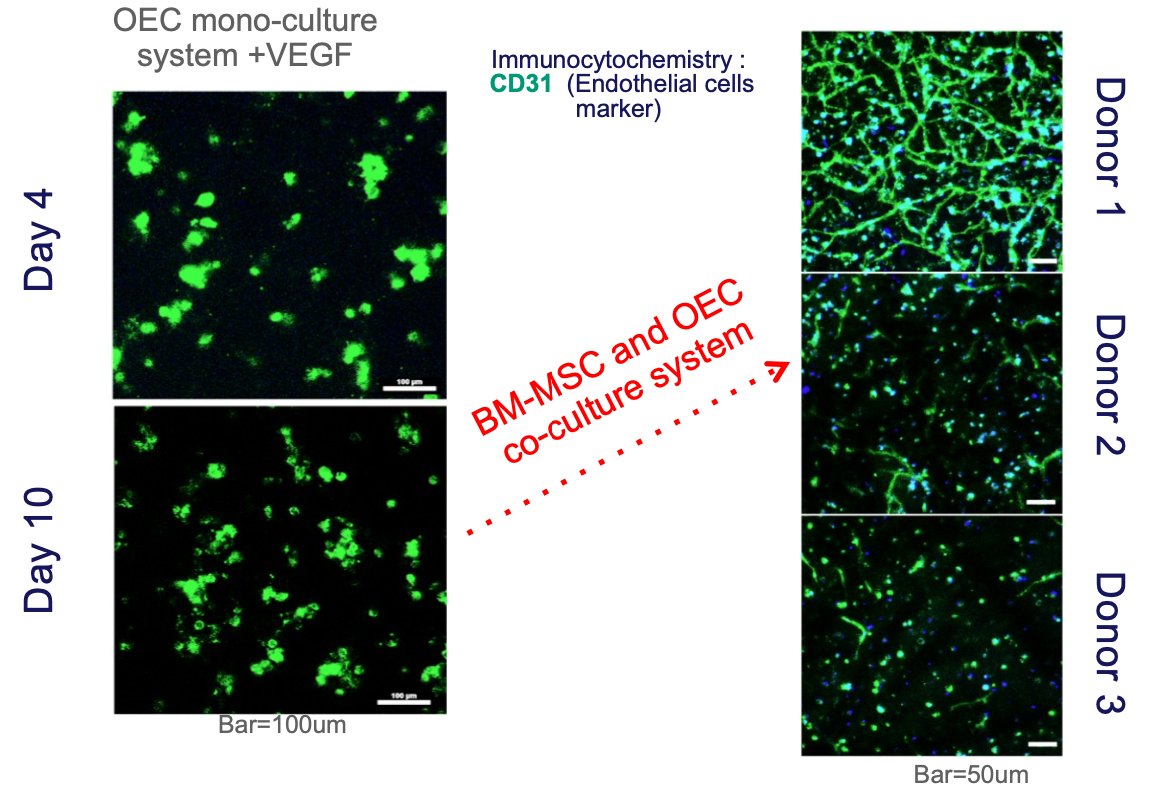
\includegraphics[width=0.5\textwidth]{coculture}
\caption{\label{fig:coculture}}
\end{figure}
\noindent
Considering the bone, the presence of two families leads to best results: osteoblast work will lead to an increase endothelial cells formation. Osteoblast cells know how much and when to release factors. Osteoblasts also produce a collagenic template used by endothelial cells to form tubes. When we take into account the scaffold, we can support the direct interaction with both osteoblast and endothelial cells. 
Example: fibroin micronet, co-cultured, 3d scaffold. The endothelial cells become tubes, there is a collagenic network.
We need that the tubes are stable. In the microscope view we can see that there is a very physiological structure. 

\section{Vascularization strategies}
New strategies to achieve better blood vessels: architecture is important, should provide something to make endothelial cell grow mechanism of angiogenesis can be amplified. Porous matrices can be loaded with growth factor, functionalization to recruit blood vessels from surrounding tissues. They should be able to penetrate and form interconnected tissue.
\\
\\
\noindent
The main vascularization strategies are:
\begin{itemize}
\item angiogenesis: ingrowth of vascular sprouts from the host microvasculature into implanted tissue construct, which finally form a new microvascular network
\item inosculation: pre-created vessels in vitro (network, not real vessels) is generated within a tissue construct prior to implantation. Connection with host vessels + already included vessels. Usually animal cells are used, in order to distinguish which vessels are new and which are implanted through staining. Sometimes scaffold tubes are not able to anastomize and die, our aim is to preserve the mixture and anastomize (circle in the picture).
\end{itemize}

\begin{figure}[h]
\centering
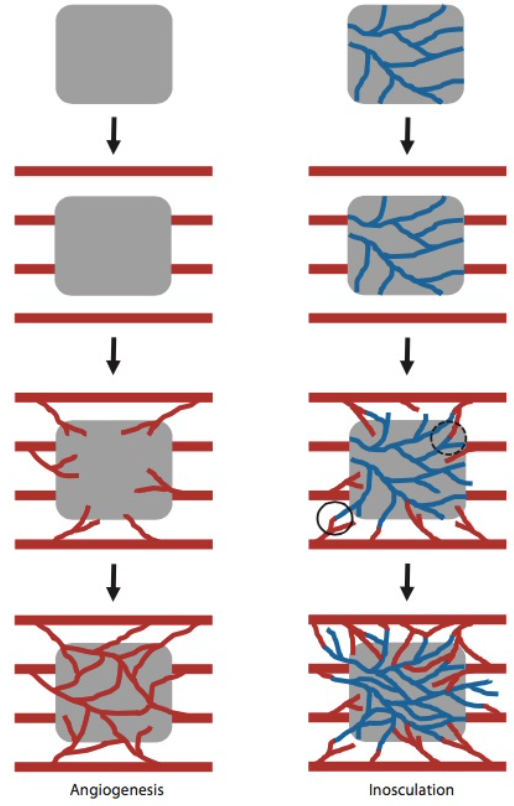
\includegraphics[width=0.3\textwidth]{vasc}
\caption{\label{fig:vasc}}
\end{figure}

\subsection{Immune response and vascularization}
We have also to remember that inflammation (immune response) induces to angiogenesis.
Initially we have the recruitment of macrophages. Granulation tissue must be vascularized.
Two different structures with different porosity. In the first case (high porosity) we have a fine granulation tissue, angiogenic factors and new vessels. After 2 weeks we have less, much less inflammatory response.  In the second case there is no vascularisation, so this is not good. There is a thick layer of fibrotic tissue.

In vivo vascularisation scaffold induced
Polymer: form a sponge with a porosity with different pore sizes. 
\begin{itemize}
\item PDLLA: blood vessels are just around (3wks)
\item PDLLAA + silk fibers: very nice capillary branch formation into the scaffold (3wks)
\end{itemize}
After 6 weeks Silk seems to be intrinsically angiogenic.
We need early and efficient angiogenesis, the winner is always the scaffold that achieves the result in a short time. Which are the intrinsic angiogenic properties of silk fibroin net and mechanism? We don’t know yet for sure, but we need them!

\begin{figure}[h]
\centering
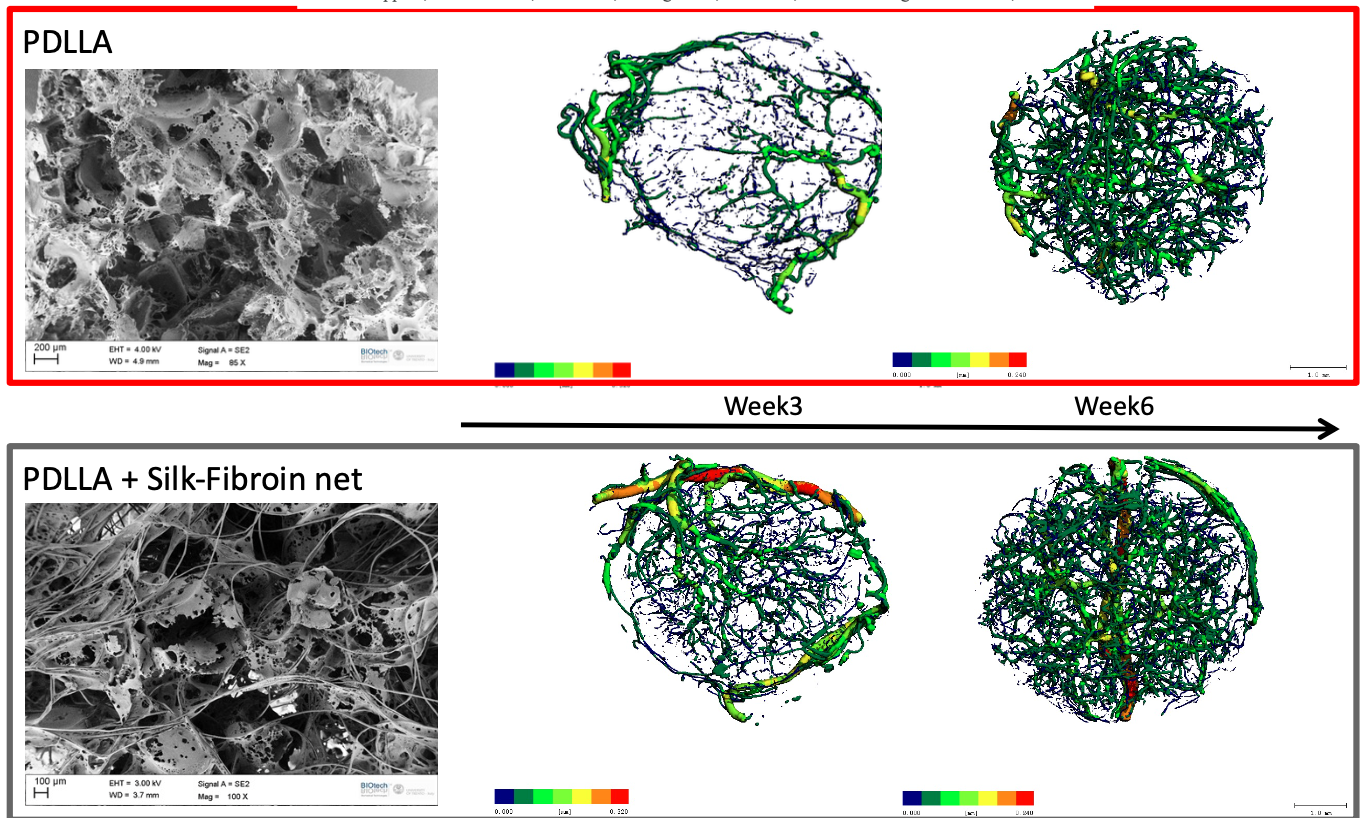
\includegraphics[width=0.5\textwidth]{pdlla}
\caption{\label{fig:pdlla}}
\end{figure}

\subsubsection{Different polymers in co-culture}
Comparison of different polymers with co-culture (HA, calcium phosphate, Ni-Ti, fibroin). The results are quite different, it’s important to carefully design the in vitro test, but it is not enough if the substrate is not specifically bioactive.

\subsubsection{Angiogenesis driven by inflammatory cells}
The fibroin net was implanted with and without pre-seeding osteoblasts. A very nice and intense angiogenesis was observes thanks to the interaction between osteoblasts and inflammatory signal.
Different pre- culture time
Manage the inflammatory response better in the case B.
Impact on angiogenesis: second scaffold has a better angiogenesis!
Drug release system works and speeds up the angiogenesis process.

\begin{figure}[h]
\centering
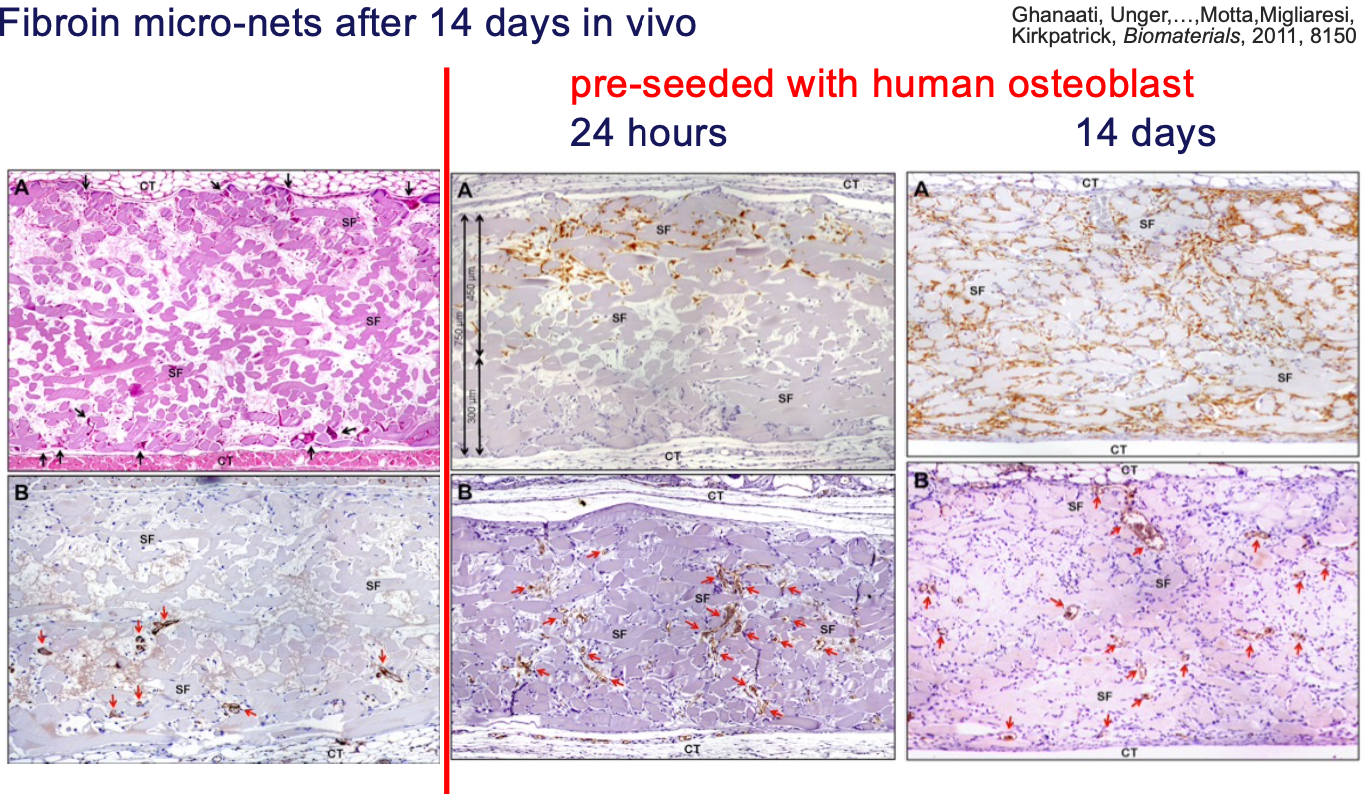
\includegraphics[width=0.5\textwidth]{fibroin}
\caption{\label{fig:fibroin}}
\end{figure}

\section{Induction of vascularization in TE scaffolds}
After the selection and dosage of the molecules we need to design how to release them into the system. 

\subsection{PDGF-containing microspheres}
Dual factor delivery from degradable scaffolds for de novo blood vessels synthesis: we can have PDGF-containing microspheres: the molecules must exit from the vescicle, move in a matrix and then release (very slow process). We need to assess degradation does not occur prior to release and whether microparticles are active and alive throughout the waiting time. 
\subsection{Cytokine delivery}
The sequential delivery of VEGF and PDGF-BB using a controlled release polymeric device subcutaneously and in hind limb ischemia model induced a mature new vascular network with vessels having a thick coat of smoot muscle cells. The combination of the two gives the best and fastest angiogenesis.
\subsection{Microparticles}
Scaffold design by microparticle assembly. Microparticles preparation:
\begin{itemize}
\item formation of microparticles via single emulsion
\item  double emulsion: with growth factors
\end{itemize}

It includes the microspheres: loaded or not with drugs.
Sintering: formation of microparticles with some porosity inside
Printing: print microparticles Single emulsion: method of sintering.

Very good adhesion with sintering process. Sintering is usually used for ? alloy, but also with polymers and ceramics.
The porosity can be improved by mixing with water (water soluble or insoluble materials).
You can also use polymers with this technology, at first this technology needed really high temperatures and so not good with polymers, but now lower temperatures are needed.

\subsection{Strategies for enhancing vascularization}
By host: with growth factors pros: easy to engineer, high quality vessels, cons: too slow
Really slow is a cons because the tissue needs to be vascularised in order to work properly.
Engineered vascular network:
pros: immediate perfusion
cons: hard to engineer, must be compatible with blood We want to provide porosity but also canals.
Also tubes can provided, for example tubes with ice, to be filled with vessels.




    \graphicspath{{chapters/bioreactors/}}
\chapter{Bioreactors}

\section{Scaffold development process}
We start from a pathology, analyze the microenvironment (not only chemical signals but also mechanical signals, ability to heal) and the tissue to regenerate. From this info we can build scaffold able to mimic the morphology. The goal must be reached by carefully designing materials and manufacturing methods. E.g. 3D printing layer by layer allows us to obtain gradients with different properties. After obtaining a scaffold we need to characterize it with biological function. Once a good result is obtained we can pass to clinical trials: first of all make sure that we are not producing damages to the body, secondly demonstrate suitability  for therapeutic purposes.

\section{3D structures}
Growing cells on flat surfaces is unnatural and artificial, it does not make sense in a biological perspective.
Natural ECM plays an important role in regulating cellular behaviours by influencing cells with biochemical signals and topographical cues.
In 3D cultures, we can control scaffold morphology, architecture and chemistry, bio recognition signaling, degradation mechanisms, patterns; cells behave and respond to stimuli more like they would do in vivo.
\\
\\
\noindent
2D culture substrates are not able to reproduce the complex and dynamic environments of the body, forcing cells to adjust to an artificial flat, rigid surface. 3D matrices or scaffolds are porous substrates that can support cell growth, organisation, and differentiation on or within their structure. Architectural and material diversity have much more impact on 3D matrices than on 2D substrates. Other than physical properties, chemical and biochemical modification with specific biological motives to facilitate cell adhesion, cell mediated proteolytic degradation and growth factor binding and release.
\\
\\
\noindent
In order to build an effective scaffold we must be very precise and stick to biological processes.  While working in vitro we must carefully choose cells e.g. monocytes to evaluate immune response. The mechanics should be dynamic, not static. We need to decide stresses to apply, their intensity and timing. Bioreactors should always be designed by keeping in mind the application.


\end{document}
